
\chapter{Developing a Bang! application with CVLiBG and Dataset Creator}
\label{bangImplementation}
This chapter starts with basic information about the card game Bang!, followed by creating a first model and an example use of the dataset tool. Next, the chapter continues with the implementation of a mobile application at a higher abstraction level, explaining the design choices.

\section{Card game Bang!}
Bang! is a western style card game for 4 to 7 players, with a suggested age of 8 or older. The game was created by Italian author Emiliano Sciarra \cite{bangWiki}, it was released in 2002 by the Italian publisher DV Giochi. In the Czech Republic and Slovak Republic, the game is released and manufactured by Albi. The game is very popular and has achieved 4 million sales worldwide.

\subsection{Rules of Bang!}
At the start of the game, players are randomly assigned one of the roles: Sheriff, Sheriff's Assistant, Bandit, or Renegade. While the game-play is the same for all roles, their end goals are different. \textbf{Sheriff's} role is to get rid of the renegade and all the bandits. The sheriff also gets bonus health; however, everybody knows who the sheriff is, while all other players keep their roles a secret. \textbf{Assistants}, unlike the sheriff, do not receive any additional bonuses, and their goal is to protect the sheriff. \textbf{Bandits}, on the other hand, are targeting all other players. Their win condition is to get rid of the Sheriff. \textbf{Renegade} is the last role and is similar to bandits. However, there can only be one Renegade, and the winning condition of this role is to win the game by getting rid of the Sheriff while the Renegade and Sheriff are the only players left in the game.

Except for the roles, players are also assigned characters. These characters modify how players play the game. For example, \textit{Lucky Duke} allows the player to look at the top two cards and choose one of them instead of drawing at random. \textit{Willy the Kid} removes the limit on how many damaging cards Bang! can be played in one round by the player. And the list goes on.

The core principle of the game is simple: attack other players, defend and heal yourself, and finally stop other players from achieving their goals while trying to achieve yours. The game can be relatively explosive, and players can be taken by surprise if other players group together and start attacking them. The game itself doesn’t stop players from lying, deceiving, and forming groups to attack certain players, which, from personal experience, makes it even trickier and more fun to play.

% ===========================================================================================

% ===========================================================================================

\section{Creating a model for Bang! card game}
This section will demonstrate the use of the dataset tool for creating a model used by the Bang! demonstrative application.

\subsection{Data gathering and annotating}
First, it is necessary to gather image data with the game cards. These can be found online or taken with a smartphone's camera. Manually annotating a few dozen images might not take too much time; however, once developers start going into the hundreds, this task might start to become overwhelming. 

To help developers with this problem, the \textbf{Dataset Creator} provides an automatic annotation functionality. This, however, requires a working object detection model capable of recognizing and detecting game objects. The recommended approach is to annotate a few examples of each game object, use synthetic data generation, and utilize this data to train the first model. This model can later be used for annotation, and while the detections might not always be precise, it should speed up the further annotation of image data.

However, it should be noted that iterating and creating newer models after annotating only a few image data might not be worth the time spent on training. Developers should find a balance based on the amount of time it takes for their machine to train one model.

\subsection{Training the models}
Before training, it is required to export the dataset. Choosing the correct settings for training is mostly a matter of trial and error, especially since the batch size and number of workers will be limited by the hardware of the computer on which the dataset tool is run. Exported datasets are in Ultralytics YOLO model format. These saved datasets can be used for training outside of the \textbf{Dataset Creator} , even by other training solutions; however, conversion might be required. The \textbf{Dataset Creator} is primarily meant for hobbyists and small developers who use their machines for training as well.

% ===========================================================================================

% ===========================================================================================

\section{Mobile Application and setting up services}
After creating a new project in the integrated development environment of the developer's choice, start by adding CVLiBG to the dependencies of the project:

The starting point of the application will be the \texttt{Application} class, and it is required to subclass the abstract \texttt{CVILIBGApplication} and implement its \texttt{registerModels()} method (see \ref{applicationClass} and \ref{DetectorResult}. The Bang! application does not use any advanced functionalities and therefore just implements this class. However, should something stop developers from using \texttt{CVILIBGApplication} as the base of their \texttt{Application} class, it is required to implement its functionalities; otherwise, the \texttt{CameraController} and other parts of the library will not work.

\subsection{Data classes for navigation and card details}
Inside the application class that inherits from \texttt{CVILIBGApplication}, create a public variable named \texttt{CardDetailsService} and \textbf{Class2LinkService} using the template \texttt{JsonAssetService}. Both of these services require data classes defining the structure of the JSON object that will be loaded: \texttt{CardDetails} and \texttt{Class2Link}, respectively. For more information on how these services work, see \ref{JsonAssetService}.

The \texttt{Class2Link} is used to convert \textbf{integer class indexes}, which are the output of \texttt{Detector}, into \textbf{string based link} identifiers that are used for navigation when displaying details for each card or symbol.

The \texttt{CardDetails} is used to define the content of the page that is displayed to the user after clicking on the detection. This data class contains a path to the image, a name, a description, and the ID of the object. The ID is a string and must be correctly linked to the class index inside the \texttt{Class2Link}.

\section{Main activity}
Android projects need an activity as a starting point. The main activity of this project will also be the only activity. This application will use fragments instead of activities. Therefore, the navigation logic can be defined only inside the main activity and shared across all fragments. This activity will contain a camera preview and therefore requires a permission request to use it; this can be achieved with \texttt{PermissionService}.

Lastly, it is necessary to change the \texttt{AndroidManifest.xml} file and add the activity and application files used by the project (see \ref{androidManifestExample} for an example of the \texttt{AndroidManifest.xml}).

% ===========================================================================================

% ===========================================================================================


\section{Fragments}
Fragments are used as small parts of the UI that can be swapped inside the activity. This approach allows to reuse navigation buttons and logic from the main activity inside the individual fragments.

\subsection{CameraFragment}
\begin{verbatim}
    override fun onViewCreated(view: View, savedInstanceState: Bundle?) {
        super.onViewCreated(view, savedInstanceState)
        
        detectionOverlay.onDetectionClicked = { detection ->
            val bundle = bundleOf("id" to class2linkService
                .items[detection.classIndex]!!.linkId)
                
            findNavController().navigate(R.id.cardDetailsFragment, bundle)
} }
\end{verbatim}

The code above is responsible for the on-click behavior of the detected objects drawn onto the screen. The \texttt{DetectionOverlay's} \texttt{onDetectionClicked} is a callback function that is executed on user interaction with detected objects (for more information, see \ref{DetectionOverlay} or \ref{BangDetectionOverlay}). The lambda function uses the \texttt{Class2LinkService} to convert the integer class value into a string link Id that is used by the navigation controller to open the details card.

Further, it is required to provide \texttt{Detector} classes for the \texttt{CameraController}, which is done by implementing the abstract \texttt{setupDetectors()} method. For this application, detectors are set up with \texttt{SettingsService} and allow users to change detectors and models in settings. The rest of the camera setup is handled by \texttt{AbstractCameraFragment}, from which this class is derived.

\begin{verbatim}
override fun setupDetectors() {
    realtimeDetector = DetectorRegistry.createDetector(
        settingsService.realtimeModel)
    realtimeDetector?.setMetricsEnabled(settingsService.showMetrics)
    realtimeDetector?.setVerboseMetricsEnabled(
        settingsService.verboseMetrics) }
\end{verbatim}


\subsection{DetailsFragment}
\label{DetailsFragment}
Details fragment loads values from the \texttt{CardDetailsService} based on the provided \texttt{linkID} string that is represented by the \texttt{id} inside the JSON object. Details for each card are loaded and displayed onto the \texttt{DetailsFragment}. This link system also allows defining other IDs in the \texttt{links} as clickable objects that move the user to another details card. While this is not directly implemented into the \textbf{CVLiBG}, it can be copied from this demonstration application. 

\begin{figure}[hbt]
	\centering
	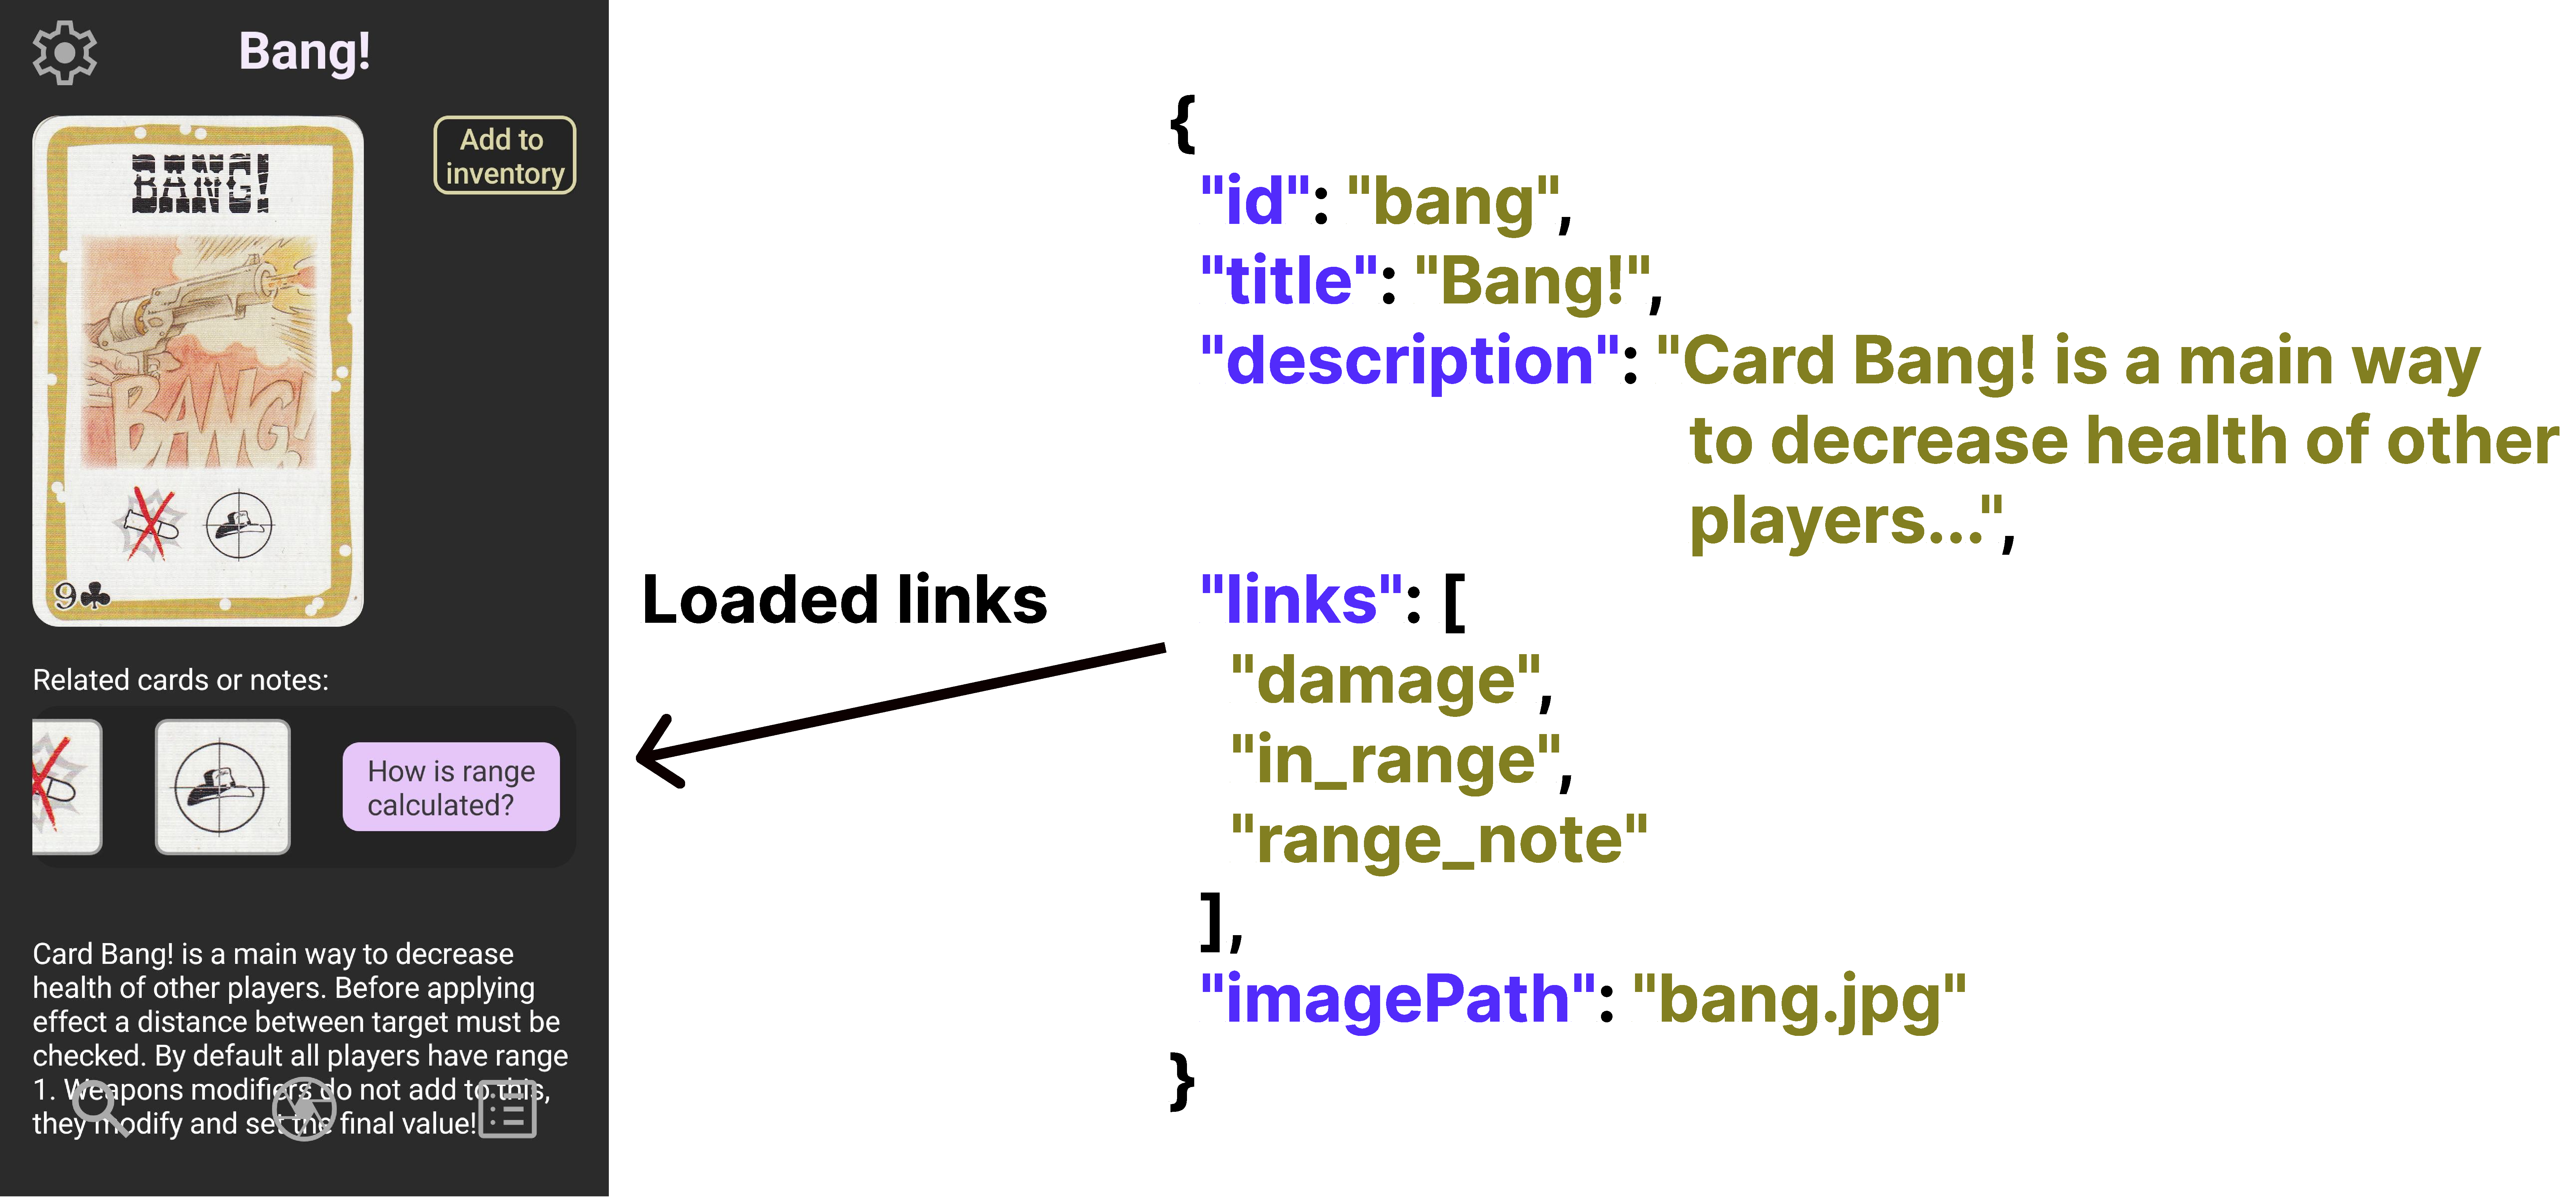
\includegraphics[width=0.98\textwidth]{obrazky-figures/DetailsFragment_scheme.pdf}
	\caption[Screenshot of fragment with card details]{Screenshot from the \texttt{DetailsFragment} with loaded Bang! card.}
	\label{DetailsFragmentScheme}
\end{figure}

\subsection{SettingsFragment}
The last fragment consists of UI elements for interacting with the \texttt{SettingsService} values, such as the application's language and the values used for selecting the object detection models.

% ===========================================================================================

% ===========================================================================================

\section{BangDetectionOverlay}
\label{BangDetectionOverlay}
The \texttt{BangDetectionOverlay} is a class derived from the \texttt{DetectionOverlay} class. It defines a \texttt{drawDetections()} method that contains code for drawing detections onto the screen. It iterates through all detection objects and uses \texttt{DetectionOverlay's} \texttt{scaleDetectionToScreenRect()} method to scale the detections properly and draw a rectangle with its name in the top left corner outside of the rectangle. 

% ===========================================================================================

% ===========================================================================================

\section{Final application}
The result application is capable of detecting objects and correctly labeling them. The camera preview is working at real-time frame-rates, and object detection can run at all times, with models trying to analyze the image as fast as possible or in a \textit{"precision"} mode that fixes the image and runs a more precise and demanding model. Models can be configured in the application's settings.

Detections are clickable and bring the users to a detailed page containing information about the card. This information is defined inside a \texttt{.json} file that is loaded from the project's assets. Details also support cross-linking between different pages that can either describe the card or a simple text based article that might explain certain edge cases for the games rules.

The application also contains simple accessibility settings for changing the font or language. The settings also contain a few options for developers who might want to change models on the fly without recompiling the project.

The whole Bang! application is written with fewer than 500 lines (excluding imports, comments, and \texttt{.xml} layouts). Most of which is UI related code.
